\documentclass{article}

\usepackage{graphicx}
\usepackage{rotating}
\usepackage{mathtools}
\DeclarePairedDelimiter{\ceil}{\lceil}{\rceil}
\DeclarePairedDelimiter{\floor}{\lfloor}{\rfloor}
\title{Obstacle Avoiding Mobile Vehicle with Rewind}
\author{Jonathan A. Garcia-Mallen}
\date{31 October 2017}

\begin{document}
\maketitle

% Is the overview just the abstract? Because that's what it is right now. 
\section*{Overview} 
% copied w/o reformatting from abstract.md
The goal is to have a robot go forward and avoid any obstacles in the way. After a certain period of time has passed, the robot will stop. Then a button can be pressed to initiate rewind. When the robot rewinds, it returns to its start pose via the same path it used to reach its end pose. Any turns it makes on the forward trip are done in reverse for the return trip. While rewinding, it performs no obstacle avoidance. To avoid obstacles, three to five [ultrasonic sensors](https://www.adafruit.com/product/3317), or three to five [IR emitters](https://www.adafruit.com/product/387) paired with [IR receivers](https://www.adafruit.com/product/157) can used as rangefinders. The robot itself can be supplied by the student.   

ADD OVERVIEW OF THIS DOCUMENT. 
\section*{System Architecture} 
THESE ARE THE FIVE THINGS
% For each subsection: 
%   inputs
%   outputs
%   what it does / its purpose

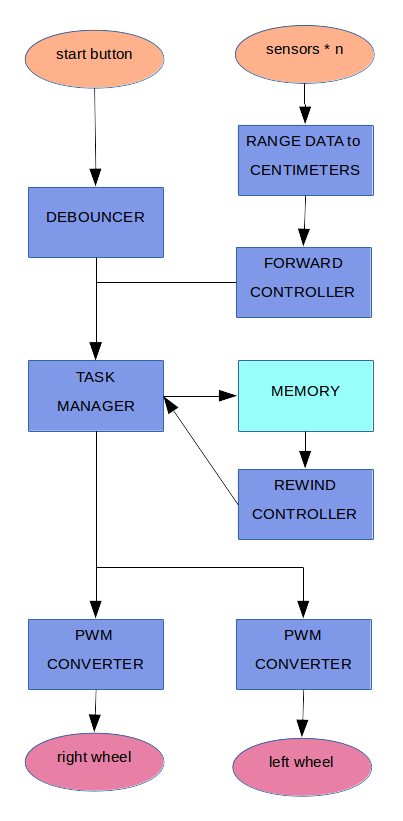
\includegraphics[width=\textwidth]{block_diagram.png}

\subsection*{System Inputs}
\subsection*{Forward Controller}
\begin{equation}
wheel\_l = speed * (\sum_{i=0}^{\floor{n/2}}{p_ir_i}) \end{equation}
\begin{equation}wheel\_r = speed * (\sum_{i=\ceil{n/2}}^{n}{p_ir_i})
\end{equation}
\subsection*{Rewind Controller and Memory}
\subsection*{PWM Converter and System Outputs}
\begin{turn}{180} 
  % system photo viewer sees an upright photo. Latex doesn't. 
  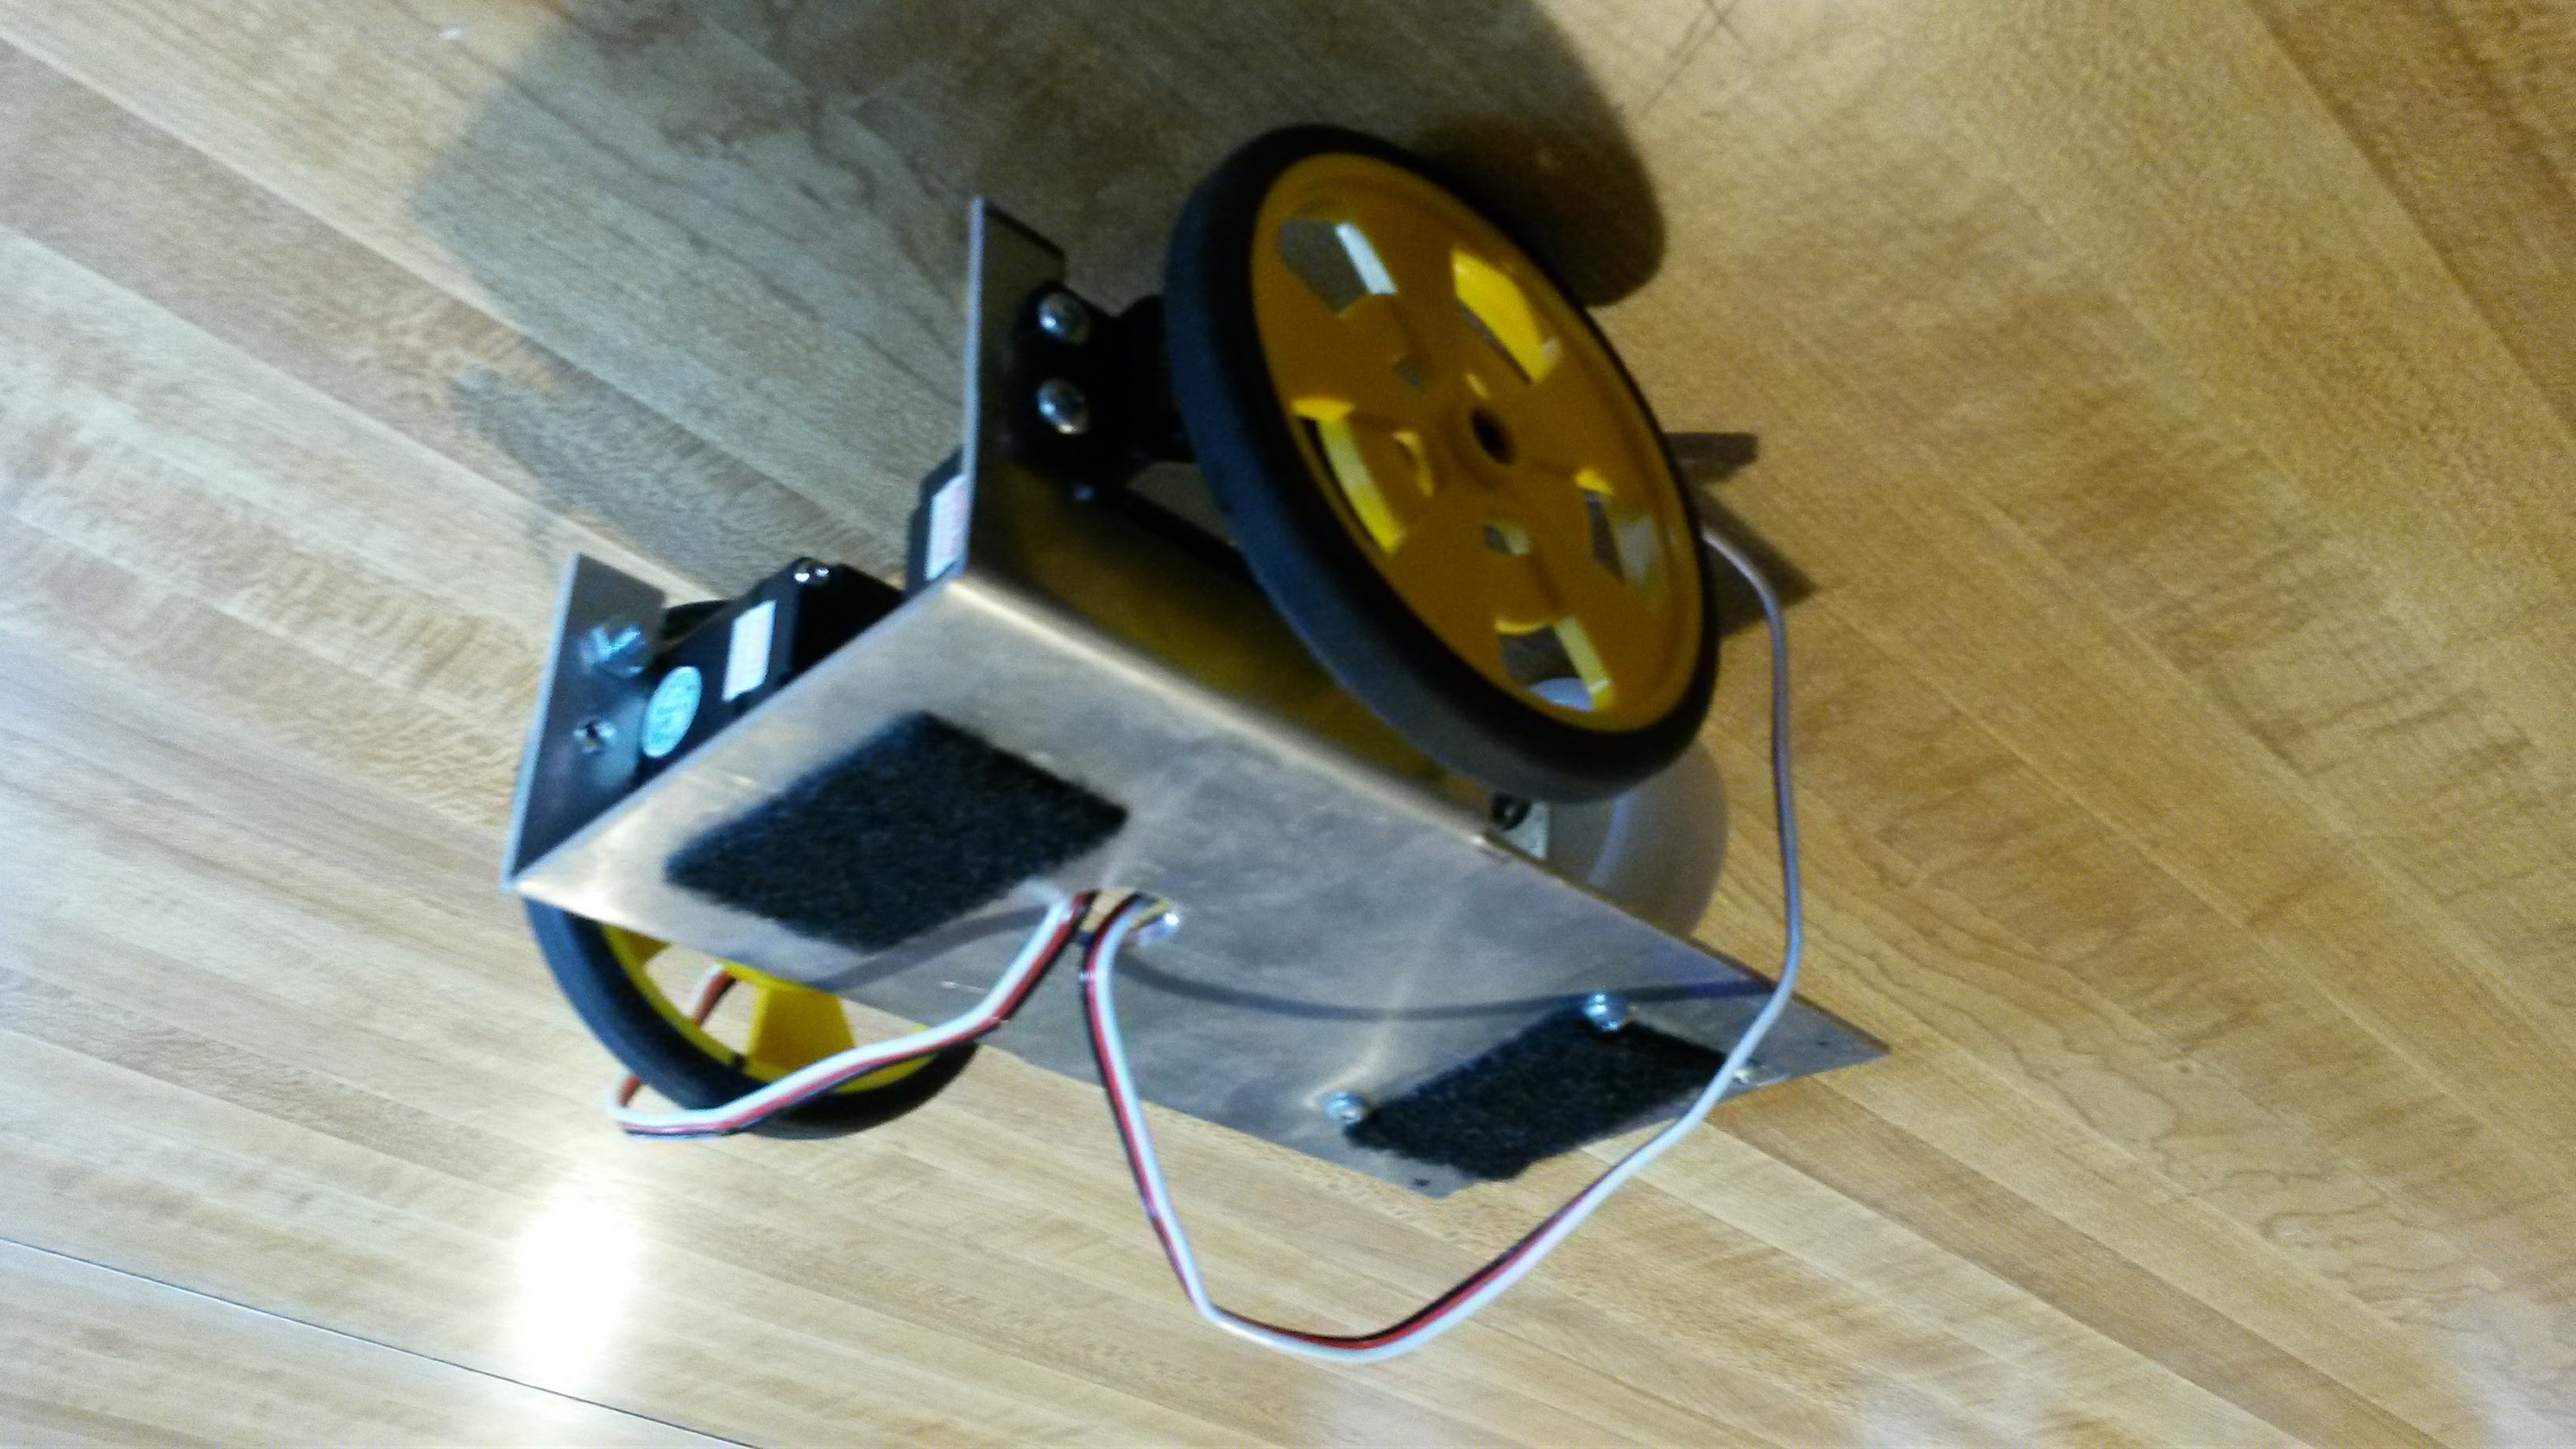
\includegraphics[width=\textwidth]{chassis.jpg}
\end{turn}
\subsection*{Task Manager} 

\section*{Complexity Analysis}

\section*{Bill of Materials}

\end{document}